\documentclass{beamer}

\usepackage{polski}
\usepackage{amsmath} %\ldots np.
\usepackage{amsfonts}
\usepackage{amssymb}
\usepackage{graphicx}
\usepackage{url}
\usepackage{tikz}
\usetikzlibrary{arrows,calc,decorations.markings,math,arrows.meta}
\usepackage{rotating}
\usepackage[percent]{overpic}
%\usepackage[cp1250]{inputenc}
\usepackage{xcolor}
\usepackage{pgfplots}
\usetikzlibrary{pgfplots.groupplots}
\usepackage{listings}
\usepackage{matlab-prettifier}
\usepackage{siunitx}
\usepackage{tabularx}
\usepackage{placeins} %\FloatBarrier
\definecolor{szary}{rgb}{0.95,0.95,0.95}
\sisetup{detect-weight,exponent-product=\cdot,output-decimal-marker={,},per-mode=symbol,range-phrase={-},range-units=single}
\SendSettingsToPgf

% Theme choice:
\usetheme{Marburg}
\usecolortheme{orchid}

% Title page details: 
\title{Dobór pętli regulacji w przypadku większej liczby sygnałów sterujących niż do wyjściowych.} 
\author{Jakub Ostrysz, Bednarz Rafał, Stankevich Stanislau}
\date{\today}
\logo{
\includegraphics[height=.5cm]{images/eiti_logo.png}}


\AtBeginSection[]
{
  \begin{frame}
    \frametitle{Spis treści}
    \tableofcontents[currentsection]
  \end{frame}
}

\pgfplotsset{compat=1.18}
\begin{document}

% Title page frame
\begin{frame}
    \titlepage 
\end{frame}

\input{Spis_treści}
% Lists frame
\section{Wprowadzenie}
\begin{frame}{Wprowadzenie}
Regulacja wielowymiarowa to proces regulacji, w którym regulowanych jest równocześnie wiele wielkości występujących w jednym obiekcie zależnych od wielu wartości sterujących.
\end{frame}

\begin{frame}{Wprowadzenie}
Rozważane algorytmy w regulacji wielowymiarowej:
\begin{itemize}
    \item PID
    \item DMC
    \item GPC
\end{itemize}
\end{frame}
\section{PID}

\begin{frame}{Wielowymiarowy PID}
Schemat projektowania wielowymiarwego algorytmu PID:
\begin{itemize}
    \item Wyznaczenie odpowiedzi skokowych wszystkich torów
    \item Przyporządkowanie najbardziej znaczącym sygnałów sterujących do wyjść
    \item Strojenie poszczególnych regulatorów
\end{itemize}
Niektóre sygnały sterujące nie będą miały wpływu na sygnały wyjściowe. 
\end{frame}


\begin{frame}{Wielowymiarowy PID}
Wyznaczenie odpowiedzi skokowych dla wszystkich torów procesu:
	\begin{center}
		\begin{figure}[H]
            		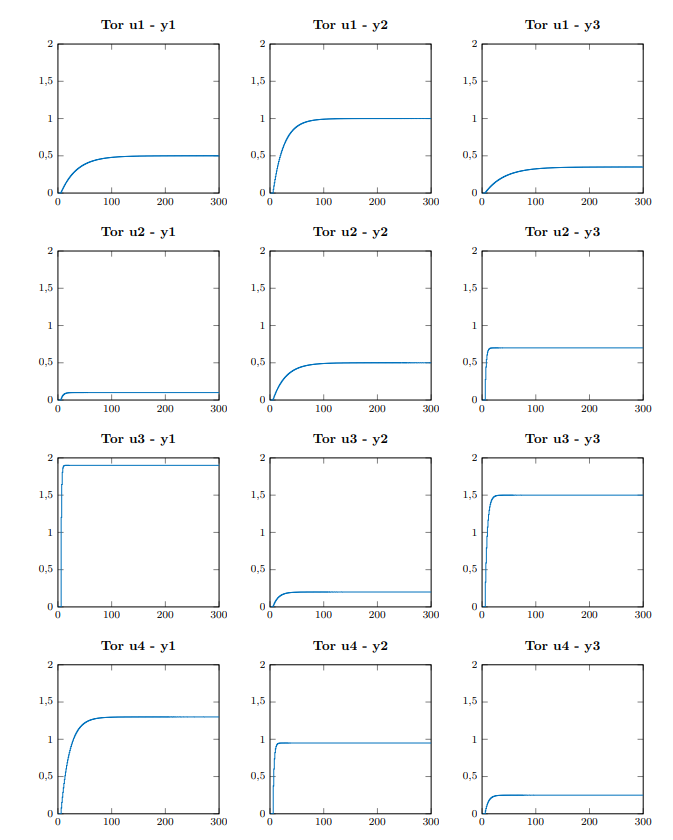
\includegraphics[scale=0.25]{images/PIDtory.png}
          			 \caption{Odpowiedzi poszczególnych torów dla skoku jednostkowego}
		\end{figure}
	\end{center}
\end{frame}

\begin{frame}{Wielowymiarowy PID}
Określenie pętli regulacji:
	\begin{center}
		\begin{figure}[H]
            		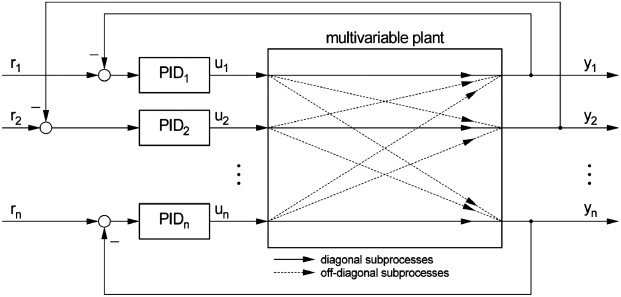
\includegraphics[scale=0.7]{images/MPID.jpg}
          			 \caption{Schemat układu regulacji}
		\end{figure}
	\end{center}
\end{frame}

\begin{frame}{Wielowymiarowy PID}
Wyniki działania:
	\begin{center}
		\begin{figure}[H]
            		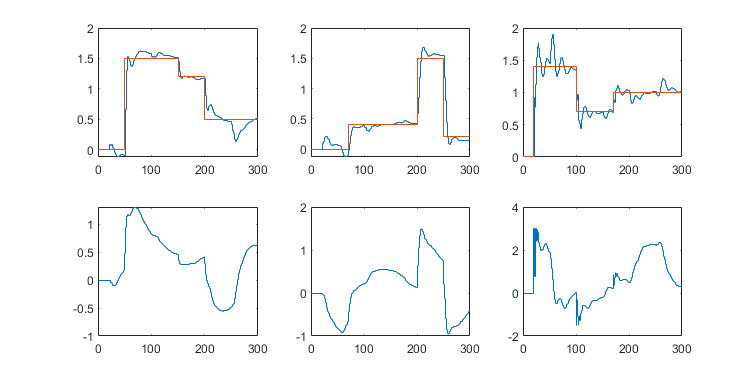
\includegraphics[scale=0.5]{images/PID_wyniki.png} %%do poprawy jak już będą ładne
          			 \caption{Wyniki regulacji}
		\end{figure}
	\end{center}
\end{frame}


% Lists frame
\section{DMC}
\begin{frame}{Wielowymiarowy DMC}
Projekt pętli regulacji z zastosowaniem wielowymiarwego algorytmu DMC:
\begin{itemize}
    \item Wyznaczenie wielowymiarowej odpowiedzi skokowej 
    \item Model w postacji odpowiedźi skokowej
    \item Rozwiązanie problemu optymalizacji
    \item Wyznaczenie wektora optymalnych przyrostów sterowań
\end{itemize}
Wszystkie sygnały sterujące wpływają na sygnały wyjściowe. 
\end{frame}


\begin{frame}{Wielowymiarowy DMC}
Wyznaczenie wielowymiarowej odpowiedzi skokowej:
	\begin{center}
		\begin{figure}[H]
            		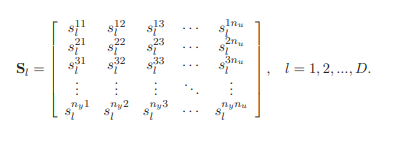
\includegraphics[scale=0.8]{images/wielowymiarowa_odp_DMC.png}
		\end{figure}
	\end{center}
\end{frame}

\begin{frame}{Wielowymiarowy DMC}
Model w postacji odpowiedzi skokowej:
	\begin{center}
		\begin{figure}[H]
            		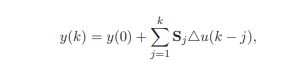
\includegraphics[scale=0.9]{images/model_DMC.png}
		\end{figure}
	\end{center}
\end{frame}

\begin{frame}{Wielowymiarowy DMC}
Rozwiązanie problemu optymalizacji:
	\begin{center}
		\begin{figure}[H]
            		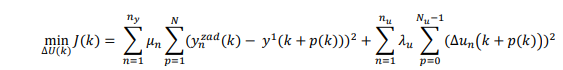
\includegraphics[scale=0.6]{images/cel_DMC.png}
		\end{figure}
	\end{center}
Zależność opisująca wyjścia przewidywane 
\begin{center}
		\begin{figure}[H]
            		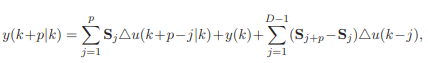
\includegraphics[scale=0.7]{images/wyjscia_DMC.png}
		\end{figure}
	\end{center}
\end{frame}

\begin{frame}{Wielowymiarowy DMC}
Określenie pętli regulacji:
	\begin{center}
		\begin{figure}[H]
            		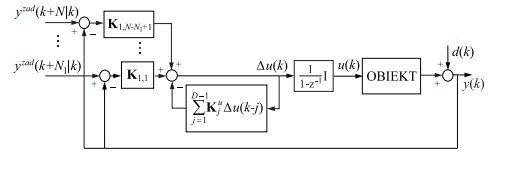
\includegraphics[scale=0.7]{images/SISODMC.png}
          			 \caption{Schemat układu regulacji}
		\end{figure}
	\end{center}
\end{frame}

\begin{frame}{Wielowymiarowy DMC}
Wyniki działania:
	\begin{center}
		\begin{figure}[H]
            		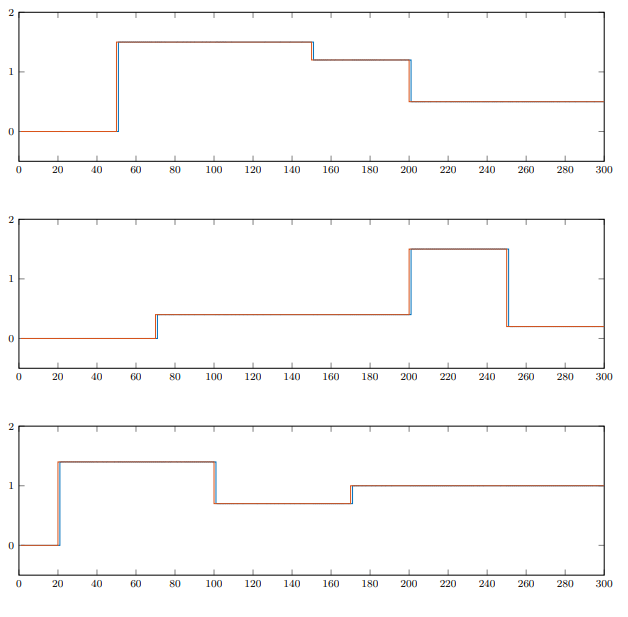
\includegraphics[scale=0.4]{images/wyniki_DMC.png} %%do poprawy jak już będą ładne
          			 \caption{Wyniki wielowymiarowej regulacji z zastosowaniem algorytmu DMC}
		\end{figure}
	\end{center}
\end{frame}

% Lists frame
\section{GPC}
\begin{frame}{Wielowymiarowy GPC}
Projekt pętli regulacji z zastosowaniem wielowymiarwego algorytmu GPC:
\begin{itemize}
    \item Wyznaczenie wielowymiarowej odpowiedzi impulsowej
    \item Model w postacji odpowiedzi skokowej
    \item Rozwiązanie problemu optymalizacji
    \item Wyznaczenie wektora optymalnych przyrostów sterowań
\end{itemize}
Wszystkie sygnały sterujące wpływają na sygnały wyjściowe. 
\end{frame}

\begin{frame}{Wielowymiarowy GPC}
Wyznaczenie wielowymiarowej odpowiedzi impulsowej:
	\begin{center}
		\begin{figure}[H]
            		
\includegraphics[scale=0.7]{images/odp_GPC.png}
		\end{figure}
	\end{center}
\end{frame}

\begin{frame}{Wielowymiarowy GPC}
Model w postacji odpowiedzi skokowej:
	\begin{center}
		\begin{figure}[H]
            		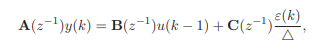
\includegraphics[scale=0.7]{images/model_GPC.png}
		\end{figure}
	\end{center}
gdzie A, B i C są macierzami wielomianowymi
\begin{center}
		\begin{figure}[H]
            		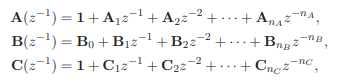
\includegraphics[scale=0.7]{images/macierze_GPC.png}
		\end{figure}
	\end{center}
\end{frame}

\begin{frame}{Wielowymiarowy GPC}
Model w przypadku działania szumów białych:
	\begin{center}
		\begin{figure}[H]
            		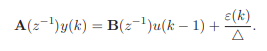
\includegraphics[scale=0.9]{images/postac_GPC.png}
		\end{figure}
	\end{center}
\end{frame}

\begin{frame}{Wielowymiarowy GPC}
Rozwiązanie problemu optymalizacji:
	\begin{center}
		\begin{figure}[H]
            		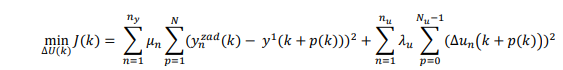
\includegraphics[scale=0.6]{images/cel_DMC.png}
		\end{figure}
	\end{center}
Zastosowanie terjektorii referencyjnej w miejsce trajektorii wartości zadanych
	\begin{center}
		\begin{figure}[H]
            		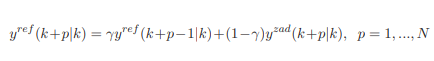
\includegraphics[scale=0.65]{images/referencyjna_GPC.png}
		\end{figure}
	\end{center}
\end{frame}


\begin{frame}{Wielowymiarowy GPC}
Określenie pętli regulacji:
	\begin{center}
		\begin{figure}[H]
            		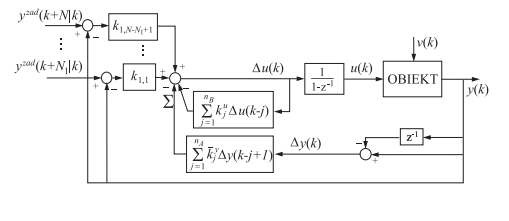
\includegraphics[scale=0.7]{images/SISOGPC.png}
          			 \caption{Schemat układu regulacji}
		\end{figure}
	\end{center}
\end{frame}

\begin{frame}{Wielowymiarowy GPC}
Wyniki działania:
	\begin{center}
		\begin{figure}[H]
            		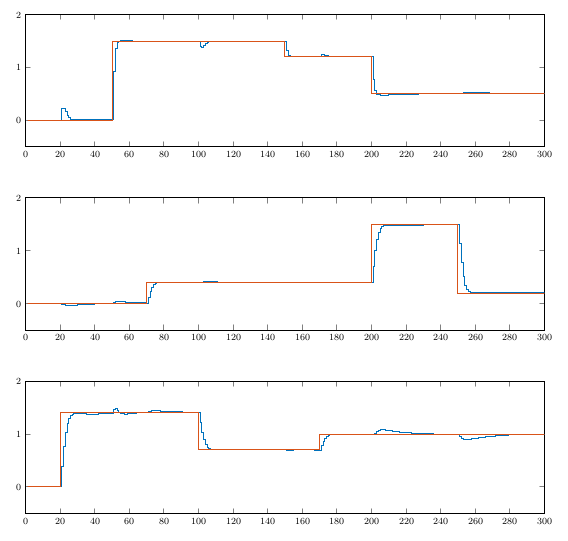
\includegraphics[scale=0.4]{images/innydmc.png} %%do poprawy jak już będą ładne
          			 \caption{Wyniki wielowymiarowej regulacji z zastosowaniem algorytmu GPC}
		\end{figure}
	\end{center}
\end{frame}

\section{Wnioski}
\begin{frame}{Wnioski}

Ocena działania poszczególnych układów wielowymiarowej regulacji:
\begin{itemize}
    \item PID
    \item DMC
    \item GPC
\end{itemize}

\end{frame}
\section{Bibliografia}
\begin{frame}{Bibliografia}
[1] P. Tatjewski. Sterowanie zaawansowane obietów przemysłowych Struktury i algorytmy. 2016 

[2] R. Dittmar, S.Gill, H. Singh, M.Darby. Robust optimization-based multi-loop PID controller tuning: A new tool and its industrial application. 2011
\end{frame}
\end{document}